% ===== backpropagation =====
\section*{Backpropagation}
% ---- CS189 scope checklist: must include ([x] = already covered) ----
% Source: Lecture 13; Discussion 7; reference sheet p.8
% [ ] Why: SGD needs the gradient of the loss for every weight
% [ ] Computation graph (forward pass computes the values)
% [ ] Chain rule along one path; sum over multiple paths
% [ ] Backward pass: adjoint a_L = 1, a_i = sum over children a_j dv_j/dv_i
% [ ] Process nodes in reverse topological order
% [ ] Matrix rules: C = AB -> G B^T, A^T G; elementwise; bias = G summed over rows
% [ ] Worked example, e.g. f(x, y, z) = (x + y) z
% ----

% draws a vertical nudge arrow: \nudge{x}{y}{signed size}{scale}{line width}
% blue up = increase, red down = decrease, nothing if 0
\newcommand{\nudge}[5]{%
  \pgfmathsetmacro{\nudgeL}{#4*(#3)}%
  \pgfmathsetmacro{\nudgeA}{#2-\nudgeL/2}%
  \pgfmathsetmacro{\nudgeB}{#2+\nudgeL/2}%
  \ifdim \nudgeL pt>0.001pt
    \draw[-stealth, blue!70!black, line width=#5] (#1,\nudgeA) -- (#1,\nudgeB);
  \else\ifdim \nudgeL pt<-0.001pt
    \draw[-stealth, red!80!black, line width=#5] (#1,\nudgeA) -- (#1,\nudgeB);
  \fi\fi}

Backpropagation computes the \textbf{gradient} of the cost, $\nabla E$: one slope per parameter (13{,}002 total). Since $E$ averages over every example, each step depends on every example, so we start with \textit{one}.

\subsection*{Desired Nudges for One Example}
\begin{keeptogether}
We continue with the handwritten-digit network from the Neural Networks section. Take one training example: an image of a 2. The network is still untrained, so the outputs are random.
\begin{itemize}
  \item We want neuron 2 to go up to 1 and every other neuron to go down to 0.
  \item Each nudge is proportional to how far that output is from its target, $t_k - \hat{y}_k$.
  \item We can't change the outputs directly (only weights and biases), but we keep track of these nudges.
\end{itemize}

{\centering
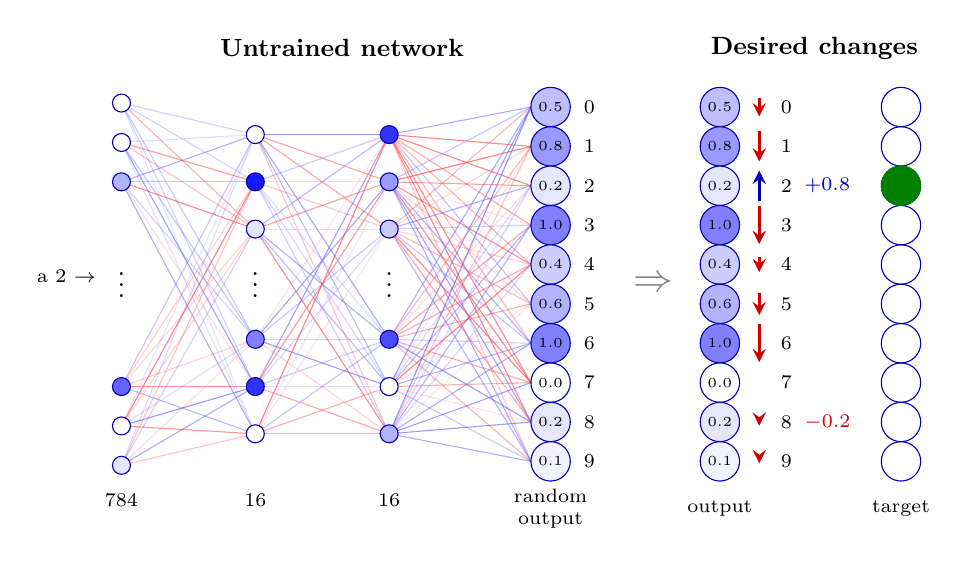
\begin{tikzpicture}[>=latex,
    nrn/.style={circle, draw=blue!70!black, minimum size=6.5pt, inner sep=0pt},
    onrn/.style={circle, draw=blue!70!black, minimum size=0.5cm, inner sep=0pt, font=\tiny}]
\pgfmathsetseed{289}
% ===== panel 1: the untrained network =====
\node[font=\small\bfseries] at (2.8,3.0) {Untrained network};
\foreach \y [count=\n] in {2.3,1.8,1.3,-1.3,-1.8,-2.3} \coordinate (a\n) at (0,\y);
\foreach \y [count=\n] in {1.9,1.3,0.7,-0.7,-1.3,-1.9} \coordinate (b\n) at (1.7,\y);
\foreach \y [count=\n] in {1.9,1.3,0.7,-0.7,-1.3,-1.9} \coordinate (c\n) at (3.4,\y);
\foreach \i in {1,...,6} \foreach \j in {1,...,6} {
  \pgfmathsetmacro{\r}{rnd}\pgfmathsetmacro{\o}{0.15+0.55*rnd}
  \ifdim\r pt<0.5pt \draw[blue!60, opacity=\o] (a\i) -- (b\j); \else \draw[red!70, opacity=\o] (a\i) -- (b\j); \fi
  \pgfmathsetmacro{\r}{rnd}\pgfmathsetmacro{\o}{0.15+0.55*rnd}
  \ifdim\r pt<0.5pt \draw[blue!60, opacity=\o] (b\i) -- (c\j); \else \draw[red!70, opacity=\o] (b\i) -- (c\j); \fi}
\foreach \i in {1,...,6} \foreach \k in {0,...,9} {
  \pgfmathsetmacro{\r}{rnd}\pgfmathsetmacro{\o}{0.15+0.55*rnd}
  \pgfmathsetmacro{\yk}{2.25-0.5*\k}
  \ifdim\r pt<0.5pt \draw[blue!60, opacity=\o] (c\i) -- (5.2,\yk); \else \draw[red!70, opacity=\o] (c\i) -- (5.2,\yk); \fi}
\foreach \n/\s in {1/0,2/0,3/30,4/60,5/0,6/10} \node[nrn, fill=blue!\s] at (a\n) {};
\node at (0,0.1) {$\vdots$};
\foreach \n/\s in {1/0,2/90,3/10,4/50,5/80,6/0} \node[nrn, fill=blue!\s] at (b\n) {};
\node at (1.7,0.1) {$\vdots$};
\foreach \n/\s in {1/80,2/40,3/20,4/70,5/0,6/30} \node[nrn, fill=blue!\s] at (c\n) {};
\node at (3.4,0.1) {$\vdots$};
\foreach \k/\v in {0/0.5, 1/0.8, 2/0.2, 3/1.0, 4/0.4, 5/0.6, 6/1.0, 7/0.0, 8/0.2, 9/0.1} {
  \pgfmathsetmacro{\y}{2.25-0.5*\k}
  \pgfmathsetmacro{\s}{50*\v}
  \node[onrn, fill=blue!\s] at (5.45,\y) {\v};
  \node[font=\scriptsize, anchor=west] at (5.75,\y) {\k};
}
\node[font=\scriptsize] at (0,-2.75) {784};
\node[font=\scriptsize] at (1.7,-2.75) {16};
\node[font=\scriptsize] at (3.4,-2.75) {16};
\node[font=\scriptsize, align=center] at (5.45,-2.85) {random\\output};
\node[font=\scriptsize, anchor=east] at (-0.2,0.1) {a 2 $\to$};
% ===== panel 2: desired changes =====
\node[font=\Large, gray] at (6.75,0) {$\Rightarrow$};
\begin{scope}[shift={(7.6,0)}]
\node[font=\small\bfseries] at (1.2,3.0) {Desired changes};
\foreach \k/\v/\n in {0/0.5/-0.5, 1/0.8/-0.8, 2/0.2/0.8, 3/1.0/-1.0, 4/0.4/-0.4, 5/0.6/-0.6, 6/1.0/-1.0, 7/0.0/0, 8/0.2/-0.2, 9/0.1/-0.1} {
  \pgfmathsetmacro{\y}{2.25-0.5*\k}
  \pgfmathsetmacro{\s}{50*\v}
  \node[onrn, fill=blue!\s] at (0,\y) {\v};
  \nudge{0.5}{\y}{\n}{0.48}{1.1pt}
  \node[font=\scriptsize, anchor=west] at (0.65,\y) {\k};
  \node[onrn] at (2.3,\y) {};
}
\node[onrn, draw=green!50!black, fill=green!50!black] at (2.3,1.25) {};
\node[font=\scriptsize, blue!70!black, anchor=west] at (0.95,1.25) {$+0.8$};
\node[font=\scriptsize, red!80!black, anchor=west] at (0.95,-1.75) {$-0.2$};
\node[font=\scriptsize] at (0,-2.85) {output};
\node[font=\scriptsize] at (2.3,-2.85) {target};
\end{scope}
\end{tikzpicture}
\par}
{\centering\scriptsize Neuron 2's $+0.8$ matters more than neuron 8's $-0.2$.\par}
\end{keeptogether}

\subsection*{Adjusting One Neuron}
\begin{keeptogether}
Zoom in on neuron 2:
\[
\hat{y}_2 = \sigma\big(w_1 h_1 + w_2 h_2 + \cdots + w_n h_n + b\big)
\]
There are three ways to raise it:
\begin{enumerate}
  \item Increase the bias $b$.
  \item Increase the weights $w_j$, \textbf{in proportion to $h_j$}: weights from bright neurons (high $h_j$) matter most.
  \item Change the activations $h_j$, \textbf{in proportion to $w_j$}: raise $h_j$ if its weight is positive, lower it if negative (bigger $|w_j|$ = bigger change).
\end{enumerate}

Example for neuron 2, with 3 neurons in the previous layer (bias fixed at $b = -1.19$):

{\centering
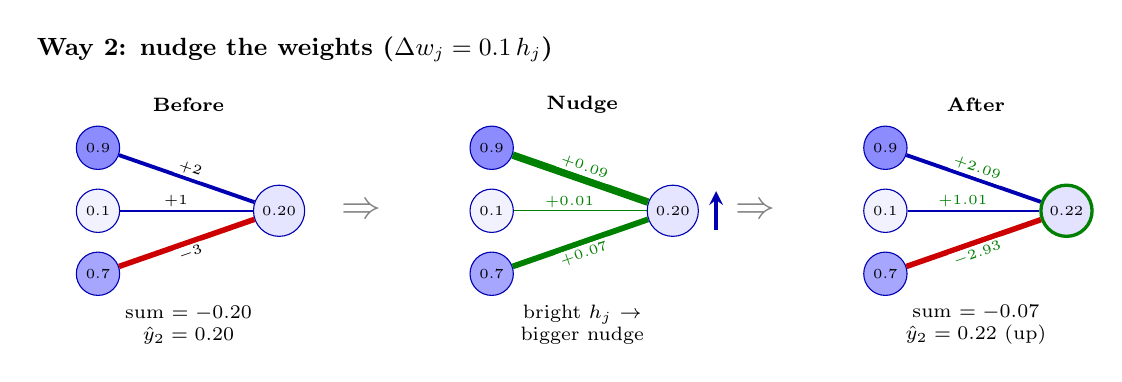
\begin{tikzpicture}[pnrn/.style={circle, draw=blue!70!black, minimum size=0.55cm, inner sep=0pt, font=\tiny}]
\node[font=\small\bfseries, anchor=west] at (-0.9,2.05) {Way 2: nudge the weights ($\Delta w_j = 0.1\, h_j$)};
\begin{scope}[shift={(0,0)}]
\node[font=\scriptsize\bfseries] at (1.15,1.35) {Before};
\node[pnrn, fill=blue!45, text=black] (n1) at (0,0.8) {0.9};
\node[pnrn, fill=blue!5, text=black] (n2) at (0,0) {0.1};
\node[pnrn, fill=blue!35, text=black] (n3) at (0,-0.8) {0.7};
\node[pnrn, minimum size=0.65cm, fill=blue!10, text=black] (o) at (2.3,0) {0.20};
\draw[blue!70!black, line width=1.4pt] (n1) -- node[above, sloped, font=\tiny, fill=white, inner sep=1pt, text=black] {$+2$} (o);
\draw[blue!70!black, line width=0.8pt] (n2) -- node[above, pos=0.42, font=\tiny, fill=white, inner sep=1pt, text=black] {$+1$} (o);
\draw[red!80!black, line width=2pt] (n3) -- node[below, sloped, font=\tiny, fill=white, inner sep=1pt, text=black] {$-3$} (o);
\node[font=\scriptsize, align=center] at (1.15,-1.45) {sum $= -0.20$\\$\hat{y}_2 = 0.20$};

\end{scope}
\begin{scope}[shift={(5,0)}]
\node[font=\scriptsize\bfseries] at (1.15,1.35) {Nudge};
\node[pnrn, fill=blue!45, text=black] (n1) at (0,0.8) {0.9};
\node[pnrn, fill=blue!5, text=black] (n2) at (0,0) {0.1};
\node[pnrn, fill=blue!35, text=black] (n3) at (0,-0.8) {0.7};
\node[pnrn, minimum size=0.65cm, fill=blue!10, text=black] (o) at (2.3,0) {0.20};
\draw[green!50!black, line width=2.7pt] (n1) -- node[above, sloped, font=\tiny, fill=white, inner sep=1pt, text=green!50!black] {$+0.09$} (o);
\draw[green!50!black, line width=0.4pt] (n2) -- node[above, pos=0.42, font=\tiny, fill=white, inner sep=1pt, text=green!50!black] {$+0.01$} (o);
\draw[green!50!black, line width=2.1pt] (n3) -- node[below, sloped, font=\tiny, fill=white, inner sep=1pt, text=green!50!black] {$+0.07$} (o);
\node[font=\scriptsize, align=center] at (1.15,-1.45) {bright $h_j$ $\to$\\bigger nudge};
\nudge{2.85}{0}{1}{0.5}{1.2pt}
\end{scope}
\begin{scope}[shift={(10,0)}]
\node[font=\scriptsize\bfseries] at (1.15,1.35) {After};
\node[pnrn, fill=blue!45, text=black] (n1) at (0,0.8) {0.9};
\node[pnrn, fill=blue!5, text=black] (n2) at (0,0) {0.1};
\node[pnrn, fill=blue!35, text=black] (n3) at (0,-0.8) {0.7};
\node[pnrn, minimum size=0.65cm, fill=blue!11, draw=green!50!black, very thick, text=black] (o) at (2.3,0) {0.22};
\draw[blue!70!black, line width=1.4pt] (n1) -- node[above, sloped, font=\tiny, fill=white, inner sep=1pt, text=green!50!black] {$+2.09$} (o);
\draw[blue!70!black, line width=0.8pt] (n2) -- node[above, pos=0.42, font=\tiny, fill=white, inner sep=1pt, text=green!50!black] {$+1.01$} (o);
\draw[red!80!black, line width=2pt] (n3) -- node[below, sloped, font=\tiny, fill=white, inner sep=1pt, text=green!50!black] {$-2.93$} (o);
\node[font=\scriptsize, align=center] at (1.15,-1.45) {sum $= -0.07$\\$\hat{y}_2 = 0.22$ (up)};

\end{scope}
\node[font=\Large, gray] at (3.35,0) {$\Rightarrow$};
\node[font=\Large, gray] at (8.35,0) {$\Rightarrow$};
\end{tikzpicture}
\par}
{\centering\scriptsize The same nudge to $w_1$ helps $9\times$ more than to $w_2$, since $h_1$ is $9\times$ brighter.\par}
\medskip
{\centering
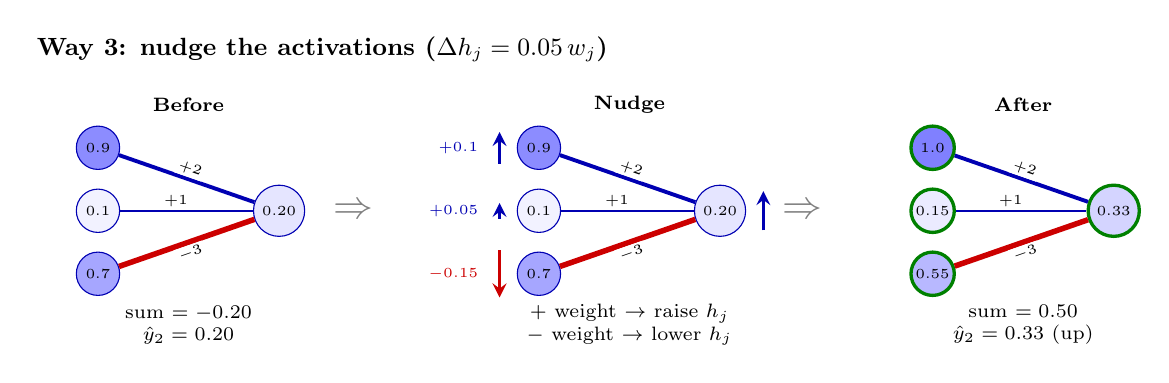
\begin{tikzpicture}[pnrn/.style={circle, draw=blue!70!black, minimum size=0.55cm, inner sep=0pt, font=\tiny}]
\node[font=\small\bfseries, anchor=west] at (-0.9,2.05) {Way 3: nudge the activations ($\Delta h_j = 0.05\, w_j$)};
\begin{scope}[shift={(0,0)}]
\node[font=\scriptsize\bfseries] at (1.15,1.35) {Before};
\node[pnrn, fill=blue!45, text=black] (n1) at (0,0.8) {0.9};
\node[pnrn, fill=blue!5, text=black] (n2) at (0,0) {0.1};
\node[pnrn, fill=blue!35, text=black] (n3) at (0,-0.8) {0.7};
\node[pnrn, minimum size=0.65cm, fill=blue!10, text=black] (o) at (2.3,0) {0.20};
\draw[blue!70!black, line width=1.4pt] (n1) -- node[above, sloped, font=\tiny, fill=white, inner sep=1pt, text=black] {$+2$} (o);
\draw[blue!70!black, line width=0.8pt] (n2) -- node[above, pos=0.42, font=\tiny, fill=white, inner sep=1pt, text=black] {$+1$} (o);
\draw[red!80!black, line width=2pt] (n3) -- node[below, sloped, font=\tiny, fill=white, inner sep=1pt, text=black] {$-3$} (o);
\node[font=\scriptsize, align=center] at (1.15,-1.45) {sum $= -0.20$\\$\hat{y}_2 = 0.20$};

\end{scope}
\begin{scope}[shift={(5.6,0)}]
\node[font=\scriptsize\bfseries] at (1.15,1.35) {Nudge};
\node[pnrn, fill=blue!45, text=black] (n1) at (0,0.8) {0.9};
\node[pnrn, fill=blue!5, text=black] (n2) at (0,0) {0.1};
\node[pnrn, fill=blue!35, text=black] (n3) at (0,-0.8) {0.7};
\node[pnrn, minimum size=0.65cm, fill=blue!10, text=black] (o) at (2.3,0) {0.20};
\draw[blue!70!black, line width=1.4pt] (n1) -- node[above, sloped, font=\tiny, fill=white, inner sep=1pt, text=black] {$+2$} (o);
\draw[blue!70!black, line width=0.8pt] (n2) -- node[above, pos=0.42, font=\tiny, fill=white, inner sep=1pt, text=black] {$+1$} (o);
\draw[red!80!black, line width=2pt] (n3) -- node[below, sloped, font=\tiny, fill=white, inner sep=1pt, text=black] {$-3$} (o);
\node[font=\scriptsize, align=center] at (1.15,-1.45) {$+$ weight $\to$ raise $h_j$\\$-$ weight $\to$ lower $h_j$};
\nudge{-0.5}{0.8}{0.1}{4}{1.2pt}
\nudge{-0.5}{0}{0.05}{4}{1.2pt}
\nudge{-0.5}{-0.8}{-0.15}{4}{1.2pt}
\node[font=\tiny, blue!70!black, anchor=east] at (-0.65,0.8) {$+0.1$};
\node[font=\tiny, blue!70!black, anchor=east] at (-0.65,0) {$+0.05$};
\node[font=\tiny, red!80!black, anchor=east] at (-0.65,-0.8) {$-0.15$};
\nudge{2.85}{0}{1}{0.5}{1.2pt}
\end{scope}
\begin{scope}[shift={(10.6,0)}]
\node[font=\scriptsize\bfseries] at (1.15,1.35) {After};
\node[pnrn, fill=blue!50, draw=green!50!black, very thick, text=black] (n1) at (0,0.8) {1.0};
\node[pnrn, fill=blue!8, draw=green!50!black, very thick, text=black] (n2) at (0,0) {0.15};
\node[pnrn, fill=blue!28, draw=green!50!black, very thick, text=black] (n3) at (0,-0.8) {0.55};
\node[pnrn, minimum size=0.65cm, fill=blue!17, draw=green!50!black, very thick, text=black] (o) at (2.3,0) {0.33};
\draw[blue!70!black, line width=1.4pt] (n1) -- node[above, sloped, font=\tiny, fill=white, inner sep=1pt, text=black] {$+2$} (o);
\draw[blue!70!black, line width=0.8pt] (n2) -- node[above, pos=0.42, font=\tiny, fill=white, inner sep=1pt, text=black] {$+1$} (o);
\draw[red!80!black, line width=2pt] (n3) -- node[below, sloped, font=\tiny, fill=white, inner sep=1pt, text=black] {$-3$} (o);
\node[font=\scriptsize, align=center] at (1.15,-1.45) {sum $= 0.50$\\$\hat{y}_2 = 0.33$ (up)};

\end{scope}
\node[font=\Large, gray] at (3.25,0) {$\Rightarrow$};
\node[font=\Large, gray] at (8.95,0) {$\Rightarrow$};
\end{tikzpicture}
\par}
{\centering\scriptsize Lowering $h_3$ helps: its weight is negative, so less gets subtracted from the sum.\par}
\end{keeptogether}

\subsection*{Propagating the Nudges Backwards}
\begin{keeptogether}
Each output neuron uses its nudge in two ways:
\begin{itemize}
  \item \textbf{Directly:} it changes its own bias and the weights feeding into it.
  \item \textbf{Through requests:} it asks the neurons in the previous layer to brighten or dim. We can't set $h_j$ directly, so each request is carried out by changing the weights and bias feeding \textit{into} $h_j$.
\end{itemize}
An output that should go up and one that should go down send opposite requests:

{\centering
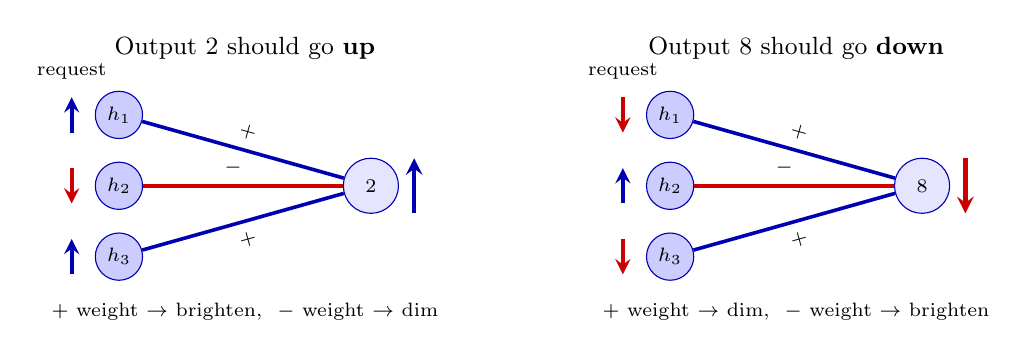
\begin{tikzpicture}[>=latex,
    hnrn/.style={circle, draw=blue!70!black, fill=blue!20, minimum size=0.6cm, inner sep=0pt, font=\scriptsize},
    onrn/.style={circle, draw=blue!70!black, fill=blue!10, minimum size=0.7cm, inner sep=0pt, font=\scriptsize}]
\foreach \ox/\title/\o/\on/\r/\cap in {
    0/{Output 2 should go \textbf{up}}/2/1/1/{$+$ weight $\to$ brighten, \ $-$ weight $\to$ dim},
    7/{Output 8 should go \textbf{down}}/8/-1/-1/{$+$ weight $\to$ dim, \ $-$ weight $\to$ brighten}} {
\begin{scope}[shift={(\ox,0)}]
\node[font=\small] at (1.6,1.75) {\title};
\node[hnrn] (h1) at (0,0.9) {$h_1$};
\node[hnrn] (h2) at (0,0) {$h_2$};
\node[hnrn] (h3) at (0,-0.9) {$h_3$};
\node[onrn] (o) at (3.2,0) {\o};
\draw[blue!70!black, line width=1.3pt] (h1) -- node[above, sloped, font=\scriptsize, black] {$+$} (o);
\draw[red!80!black, line width=1.3pt] (h2) -- node[above, font=\scriptsize, black, pos=0.45] {$-$} (o);
\draw[blue!70!black, line width=1.3pt] (h3) -- node[below, sloped, font=\scriptsize, black] {$+$} (o);
\nudge{3.75}{0}{\on}{0.7}{1.6pt}
\nudge{-0.6}{0.9}{\r}{0.45}{1.4pt}
\nudge{-0.6}{0}{-\r}{0.45}{1.4pt}
\nudge{-0.6}{-0.9}{\r}{0.45}{1.4pt}
\node[font=\scriptsize] at (-0.6,1.45) {request};
\node[font=\scriptsize] at (1.6,-1.6) {\cap};
\end{scope}}
\end{tikzpicture}
\par}
{\centering\scriptsize Going down is the same as going up with every sign flipped.\par}
\end{keeptogether}

\begin{keeptogether}
Each neuron $h_j$ in the second-to-last layer adds up the requests it receives from all the outputs. The result is $h_j$'s nudge: how much its \textit{activation} should go up or down.
\[
\text{nudge to } h_j \;\propto\; \sum_{k=0}^{9} W_{kj}\,(t_k - \hat{y}_k) \qquad (W_{kj} = \text{weight connecting } h_j \text{ to output } k)
\]
For example, one $h_j$ (ignoring the sigmoid's slope):

{\centering
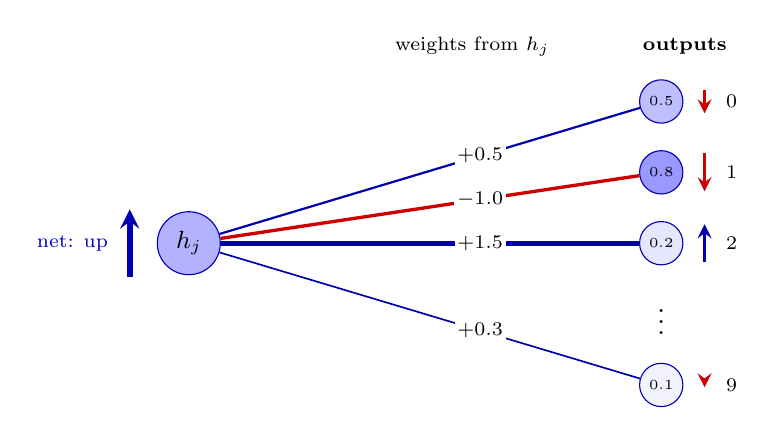
\begin{tikzpicture}[>=latex,
    onrn/.style={circle, draw=blue!70!black, minimum size=0.55cm, inner sep=0pt, font=\tiny}]
\node[circle, draw=blue!70!black, fill=blue!30, minimum size=0.8cm, font=\small] (h) at (0,0) {$h_j$};
\foreach \k/\y/\v/\n/\w/\wc/\lw in {
    0/1.8/0.5/-0.5/+0.5/blue!70!black/0.8pt,
    1/0.9/0.8/-0.8/-1.0/red!80!black/1.2pt,
    2/0/0.2/0.8/+1.5/blue!70!black/1.8pt,
    9/-1.8/0.1/-0.1/+0.3/blue!70!black/0.6pt} {
  \pgfmathsetmacro{\s}{50*\v}
  \node[onrn, fill=blue!\s] (o\k) at (6,\y) {\v};
  \nudge{6.55}{\y}{\n}{0.6}{1.2pt}
  \node[font=\scriptsize, anchor=west] at (6.7,\y) {\k};
  \draw[\wc, line width=\lw] (h) -- node[pos=0.62, fill=white, inner sep=1pt, font=\scriptsize, text=black] {$\w$} (o\k);
}
\node at (6,-0.9) {$\vdots$};
\node[font=\scriptsize\bfseries] at (6.3,2.5) {outputs};
\node[font=\scriptsize] at (3.6,2.5) {weights from $h_j$};
\nudge{-0.75}{0}{1.72}{0.5}{2pt}
\node[font=\scriptsize, blue!70!black, anchor=east] at (-0.9,0) {net: up};
\end{tikzpicture}
\par}
\[
\text{nudge to } h_j \propto \underbrace{(0.5)(-0.5)}_{\text{output 0}} + \underbrace{(-1.0)(-0.8)}_{\text{output 1}} + \underbrace{(1.5)(0.8)}_{\text{output 2}} + \cdots + \underbrace{(0.3)(-0.1)}_{\text{output 9}} > 0 \;\Rightarrow\; h_j \text{ up}
\]
\end{keeptogether}

\begin{keeptogether}
Now each $h_j$ has its own up or down nudge, just like the outputs did. So it becomes the new ``output'' and the same process repeats one layer back, until we reach the input:

{\centering
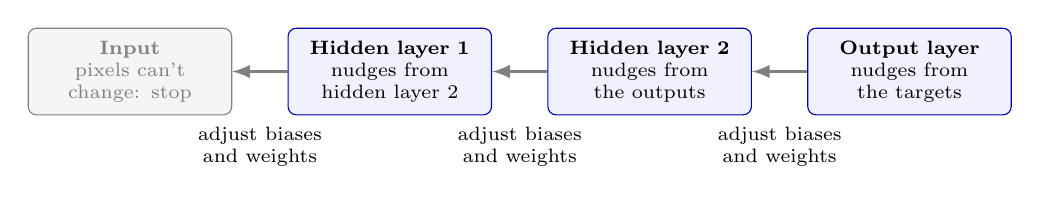
\begin{tikzpicture}[>=latex,
    box/.style={draw=blue!70!black, rounded corners=3pt, fill=blue!6, align=center, font=\scriptsize, minimum height=1.1cm, text width=2.35cm}]
\node[box] (o)  at (0,0)    {\textbf{Output layer}\\nudges from\\the targets};
\node[box] (h2) at (-3.3,0) {\textbf{Hidden layer 2}\\nudges from\\the outputs};
\node[box] (h1) at (-6.6,0) {\textbf{Hidden layer 1}\\nudges from\\hidden layer 2};
\node[box, draw=gray, fill=gray!8, text=gray] (in) at (-9.9,0) {\textbf{Input}\\pixels can't\\change: stop};
\draw[->, very thick, gray] (o) -- (h2);
\draw[->, very thick, gray] (h2) -- (h1);
\draw[->, very thick, gray] (h1) -- (in);
\node[font=\scriptsize, align=center] at (-1.65,-0.95) {adjust biases\\and weights};
\node[font=\scriptsize, align=center] at (-4.95,-0.95) {adjust biases\\and weights};
\node[font=\scriptsize, align=center] at (-8.25,-0.95) {adjust biases\\and weights};
\end{tikzpicture}
\par}
\end{keeptogether}

\subsection*{Averaging Over All Examples}
\begin{keeptogether}
So far, this is only how one training example wants to nudge the weights and biases:
\begin{itemize}
  \item \textbf{Problem:} if we only listened to it, the network would learn to classify everything as a 2.
  \item \textbf{Fix:} run the same backprop routine on every training example and record how each one wants to change the weights and biases.
  \item \textbf{Result:} average those nudges for each weight and bias.
\end{itemize}

{\centering
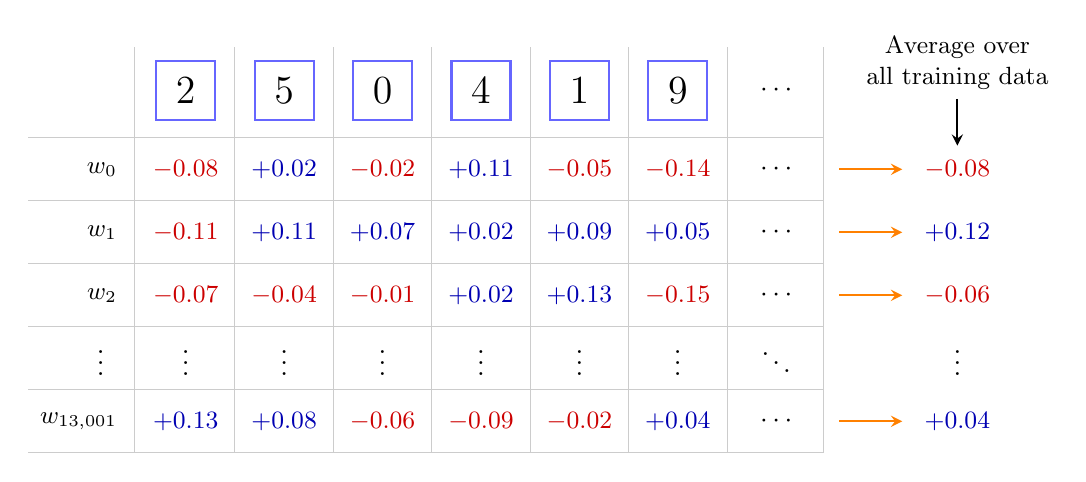
\begin{tikzpicture}[x=1cm, y=1cm]
\def\cell#1#2#3{%
  \pgfmathsetmacro{\v}{#3}%
  \ifdim \v pt<0pt \node[font=\small, red!80!black] at (#1,#2) {$#3$};
  \else \node[font=\small, blue!70!black] at (#1,#2) {$+#3$}; \fi}
% header: one column per training example
\foreach \d [count=\i from 0] in {2,5,0,4,1,9} {
  \pgfmathsetmacro{\x}{1.5+1.25*\i}
  \node[draw=blue!60, thick, minimum size=0.75cm, font=\Large] at (\x,1.0) {\d};
}
\node at (9.0,1.0) {$\cdots$};
% grid
\foreach \y in {0.4,-0.4,-1.2,-2.0,-2.8,-3.6} \draw[gray!40] (-0.5,\y) -- (9.6,\y);
\foreach \x in {0.85,2.125,3.375,4.625,5.875,7.125,8.375,9.6} \draw[gray!40] (\x,1.55) -- (\x,-3.6);
% rows
\foreach \name/\y/\a/\b/\c/\d/\e/\f/\avg in {
    w_0/0/-0.08/0.02/-0.02/0.11/-0.05/-0.14/-0.08,
    w_1/-0.8/-0.11/0.11/0.07/0.02/0.09/0.05/0.12,
    w_2/-1.6/-0.07/-0.04/-0.01/0.02/0.13/-0.15/-0.06,
    w_{13{,}001}/-3.2/0.13/0.08/-0.06/-0.09/-0.02/0.04/0.04} {
  \node[font=\small, anchor=east] at (0.75,\y) {$\name$};
  \foreach \v [count=\i from 0] in {\a,\b,\c,\d,\e,\f} {
    \pgfmathsetmacro{\x}{1.5+1.25*\i}
    \cell{\x}{\y}{\v}
  }
  \node at (9.0,\y) {$\cdots$};
  \draw[-stealth, thick, orange] (9.8,\y) -- (10.6,\y);
  \cell{11.3}{\y}{\avg}
}
\foreach \x in {0.42,1.5,2.75,4,5.25,6.5,7.75,11.3} \node at (\x,-2.35) {$\vdots$};
\node at (9.0,-2.35) {$\ddots$};
% label for the averaged column
\node[font=\small, align=center] (lab) at (11.3,1.35) {Average over\\all training data};
\draw[-stealth, thick] (lab.south) -- (11.3,0.3);
\end{tikzpicture}
\par}
Stacked into one column, the averaged nudges are the gradient descent step $-\eta\,\nabla E$ from the Neural Networks section:
\[
-\eta\,\nabla E(w_0, w_1, \dots, w_{13{,}001}) \;=\;
\begin{bmatrix} \textcolor{red!80!black}{-0.08} \\ \textcolor{blue!70!black}{+0.12} \\ \textcolor{red!80!black}{-0.06} \\ \vdots \\ \textcolor{blue!70!black}{+0.04} \end{bmatrix}
\begin{matrix} \leftarrow w_0 \\ \leftarrow w_1 \\ \leftarrow w_2 \\ \\ \leftarrow w_{13{,}001} \end{matrix}
\]
\end{keeptogether}

\subsection*{Mini-Batch Stochastic Gradient Descent}
\begin{keeptogether}
Running backprop on every training example for every single step is slow. In practice (see the Gradient Descent section):
\begin{itemize}
  \item \textbf{Split:} shuffle the training data and split it into \textbf{mini-batches} (e.g.\ 100 examples each).
  \item \textbf{Step:} compute each step from one mini-batch instead of all the data.
\end{itemize}

{\centering
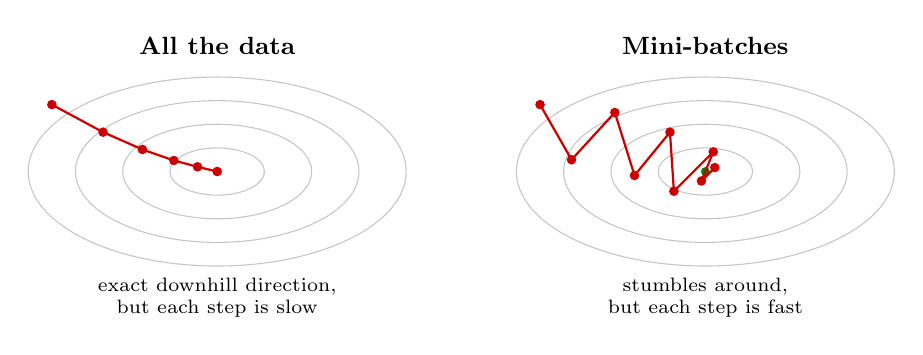
\begin{tikzpicture}
\foreach \ox/\title in {0/{All the data}, 6.2/{Mini-batches}} {
\begin{scope}[shift={(\ox,0)}]
\node[font=\small\bfseries] at (0,1.6) {\title};
\foreach \r in {1,0.75,0.5,0.25} \draw[gray!45] (0,0) ellipse ({2.4*\r} and {1.2*\r});
\fill[green!50!black] (0,0) circle (1.6pt);
\end{scope}}
% full gradient: careful, slow steps straight downhill
\draw[red!80!black, thick, mark=*, mark size=1.3pt] plot coordinates {(-2.1,0.85) (-1.45,0.5) (-0.95,0.28) (-0.55,0.14) (-0.25,0.06) (0,0)};
\node[font=\scriptsize, align=center] at (0,-1.6) {exact downhill direction,\\but each step is slow};
% mini-batch SGD: quick, stumbling steps
\begin{scope}[shift={(6.2,0)}]
\draw[red!80!black, thick, mark=*, mark size=1.3pt] plot coordinates {(-2.1,0.85) (-1.7,0.15) (-1.15,0.75) (-0.9,-0.05) (-0.45,0.5) (-0.4,-0.25) (0.1,0.25) (-0.05,-0.12) (0.12,0.05)};
\node[font=\scriptsize, align=center] at (0,-1.6) {stumbles around,\\but each step is fast};
\end{scope}
\end{tikzpicture}
\par}
Each mini-batch step only approximates the true gradient, but it's much faster: like stumbling quickly downhill instead of carefully calculating every step.
\end{keeptogether}

\subsection*{The Full Training Loop}
\begin{keeptogether}
Putting everything together:

{\centering
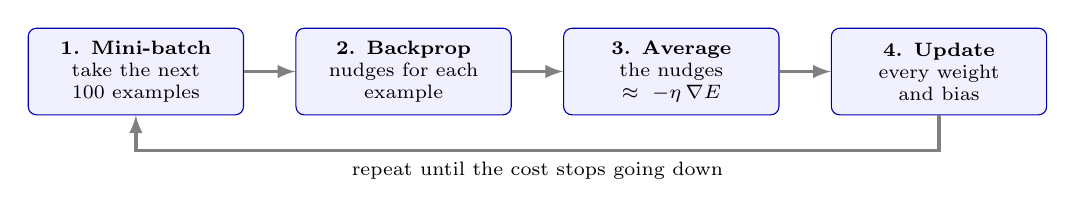
\begin{tikzpicture}[>=latex,
    box/.style={draw=blue!70!black, rounded corners=3pt, fill=blue!6, align=center, font=\scriptsize, minimum height=1.1cm, text width=2.5cm}]
\node[box] (a) at (0,0)    {\textbf{1. Mini-batch}\\take the next\\100 examples};
\node[box] (b) at (3.4,0)  {\textbf{2. Backprop}\\nudges for each\\example};
\node[box] (c) at (6.8,0)  {\textbf{3. Average}\\the nudges\\$\approx -\eta\,\nabla E$};
\node[box] (d) at (10.2,0) {\textbf{4. Update}\\every weight\\and bias};
\draw[->, very thick, gray] (a) -- (b);
\draw[->, very thick, gray] (b) -- (c);
\draw[->, very thick, gray] (c) -- (d);
\draw[->, very thick, gray] (d.south) -- ++(0,-0.45) -| node[pos=0.25, below, font=\scriptsize, black] {repeat until the cost stops going down} (a.south);
\end{tikzpicture}
\par}
Repeating this, the cost settles into a local minimum, so the network does well on the training examples. This only works with a lot of \textbf{labeled} training data, like the MNIST database of handwritten digits.
\end{keeptogether}